\section{MODELING}

In this section, we describe the thrust model and control model of a basic flapping-wing drone.

\subsection{Thrust}

\begin{figure}[thpb]
    \centering
    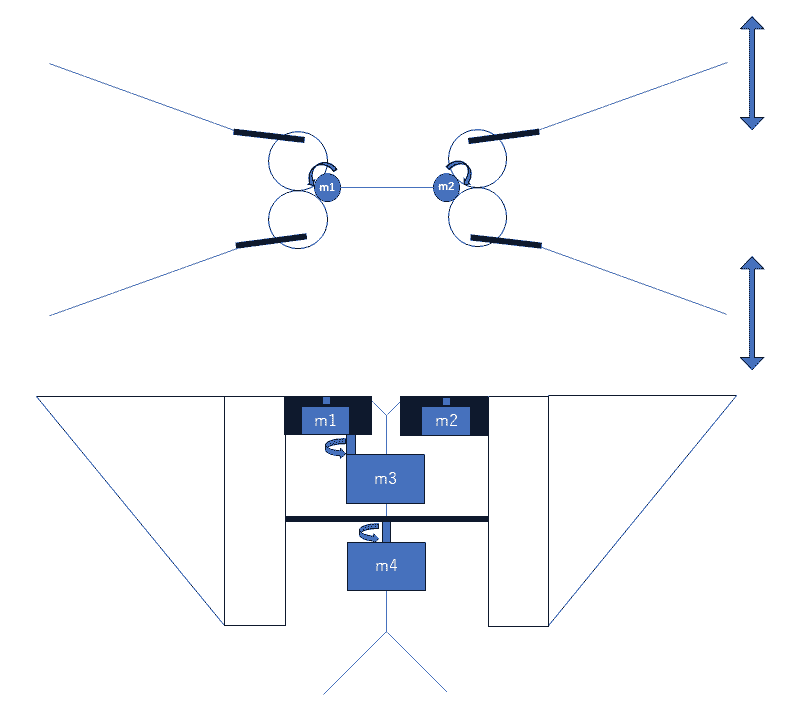
\includegraphics[width=\columnwidth]{modeling.png}
    \caption{The mechanical structure model of a flapping-wing drone. It has motors for thrust (m1, m2), a motor for wing orientation (m3), and a motor for yaw control (m4).}
    \label{figure:label}
  \end{figure}
  

Based on the model depicted in Fig. 3, the threedimensional force $f_i$ generated by $m_i$ can be
written as:

\begin{equation}
    {}^{\{CoG\}}\bm{f_i} = {\lambda_i}^{\{CoG\}}\bm{u_i},
    \end{equation}
    
    \begin{equation}
    {}^{\{CoG\}}\bm{u_i} = {}^{\{CoG\}}R_{\{F_i\}}(\phi_i, \theta_i)
    \begin{bmatrix}
    0 \\
    0 \\
    1
    \end{bmatrix},
    \end{equation}
    
    where ${}^{\{CoG\}}R_{\{F_i\}}(q, \phi_i, \theta_i)$ is the rotation matrix of the motor frame
   {\{$F_i$\}} w.r.t. the frame ${\{CoG\}}$, and $\lambda_i$ is the thrust coefficient of the $m_i$. 
   $\phi_i$ and $\theta_i$ are rotational angles of the $m_3$ and $m_4$, respectively.
   The total force and torque generated by $m_1$ and $m_2$ can be written as:
    
    \begin{equation}
    \begin{bmatrix}
    {}^{\{CoG\}}\bm{f}_\lambda \\
    {}^{\{CoG\}}\bm{\tau}_\lambda
    \end{bmatrix}
    =
    \begin{bmatrix}
    \sum_{i=1}^{2} {}^{\{CoG\}}\bm{f}_i \\
    \sum_{i=1}^{2} {}^{\{CoG\}}\bm{p}_i \times {}^{\{CoG\}}\bm{f}_i
    \end{bmatrix}
    = Q\bm{\lambda},
    \end{equation}
    
    \begin{equation}
    Q =
    \begin{bmatrix}
    {}^{\{CoG\}}u_1 & {}^{\{CoG\}}u_{2} \\
    {}^{\{CoG\}}p_1 \times {}^{\{CoG\}}u_1 & {}^{\{CoG\}}p_{2} \times {}^{\{CoG\}}u_{2}
    \end{bmatrix},
    \end{equation}
    \begin{equation}
    \lambda =
    \begin{bmatrix}
    \lambda_1 \\
    \lambda_2 \\
    \end{bmatrix}.
    \end{equation}
    

\subsection{Control}


The template is used to format your paper and style the text. All margins, column widths, line spaces, and text fonts are prescribed; please do not alter them. You may note peculiarities. For example, the head margin in this template measures proportionately more than is customary. This measurement and others are deliberate, using specifications that anticipate your paper as one part of the entire proceedings, and not as an independent document. Please do not revise any of the current designations
